\documentclass[12pt]{article}
\usepackage[margin=0.5in]{geometry}
\usepackage{titling}
\usepackage[compact]{titlesec}
\usepackage{graphicx}
\usepackage{float}
\floatplacement{figure}{H}

\setlength{\droptitle}{-4em}
\addtolength{\droptitle}{-4pt}

\title{Automatic Coffee Pot}
\author{Max Thrun}

\begin{document}
\maketitle


\section{Requirements}
\begin{itemize}
    \item Ability to set start time on a 24-hour clock
    \item When brew cycle is complete:
        \begin{itemize}
                \item Reduce the temperature to warming
                \item Indicate completion
        \end{itemize}
    \item Stop water flow if the pot is removed from its receptacle
\end{itemize}


\section{Specification}

\subsection{System Description}
This specification describes and defines the basic requirements for a automatic coffee pot. The coffee pot is able to set a brew start time on a 24-hour clock, reduce the temperature to warming when brew is complete, announce the completion of the brew, and stop the water flow if the pot is removed from its receptacle. The coffee pot is intended for daily home use by average consumers.

\subsection{Specification of External Environment}
The coffee pot is to operate in a consumer home environment in standard temperature and lighting conditions. The unit will be strickly line powered and will not contain any time of battery power. Additionally, the coffee pot will also be exposed to moisture from possible near by kitchen sinks. The unit should be fairly resistant to cleaning sprays and other types of kitchen maintance products.

\subsection{System Input and Output Specification}

\subsubsection{System Inputs}
Inputs to the system will include:
\begin{itemize}
    \item The current time of day
    \item The start brewing time set by the user
    \item The mode of operation ("Setting Brew Time" or "Running")
\end{itemize}
{\small (A 'pot removed' input is not needed as shutting off the water will be a pure mechanical solution)}

\subsubsection{System Outputs}
Depending on the current mode the system shall display either of the following on 4 7-segment displays:
\begin{itemize}
    \item The current time of day
    \item The currently set brew start time 
\end{itemize}
The brew completion signal will be indicated by an LED.

\subsection{User Interface}
The system will have three main input buttons:
\begin{itemize}
    \item \textbf{Mode Toggle:} Toggles between
        \begin{itemize}
            \item Setting brew time (Display will blink to indicate this mode)
            \item Running, where the current time of day is displayed and the unit will brew coffee when the brew time is reached.
        \end{itemize}
    \item \textbf{Increment Hour:} Increment hour when setting brew time
    \item \textbf{Increment Minute:} Increment minute when setting brew time.
\end{itemize}
Four 7-segment displays will be used to display either the set brew time or the current time of day in 24 hour format.\\
A single red LED will indicate cycle completion.

\subsection{Use Cases}
The use case for the automatic coffee pot is shown in the following diagram:
\begin{figure}
\centering
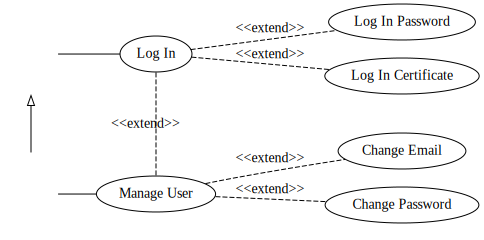
\includegraphics[scale=0.7]{use_case.png}
\caption{Use Case Diagram}
\label{fig:use_case}
\end{figure}
\begin{itemize}
    \item \textbf{Toggle Mode} The use toggles the mode into either "Setting Brew Time" or "Running".
    \item \textbf{Set Brewing Time} The user is currently setting the brew start time. The time is displayed real time on the 4 7-segment displays as it is entered. If the hour is incremented past 23 it rolls back to 0. If the minute is incremented past 59 it rolls back to 0. The selected brew time is entered by toggling the system back to the "Running" state.
    \item \textbf{Read Current Time} During normal running operation the current time of day is displayed on the 4 7-segment displays.
    \item \textbf{Read Completion Indicator} When the brew cycle is complete it is indicated to the user via a LED. The indicator is turned off when the pot is removed.
    \item \textbf{Remove Pot} When the pot is removed a mechanic mechanism shuts off the water drip.
\end{itemize}

\subsection{System Functional Specification}
The system functionality of the automatic coffee pot can be broken down in the following:
\begin{itemize}
    \item \textbf{Mode Input:} A single momentary push button will be used to toggle between the two modes.
    \item \textbf{Brew Time Input: } Two momentary push buttons, one for hour and one for minute, will be used to increment and brew time. The brew time will roll over if it exceeds 23:59.
    \item \textbf{Real Time Clock (RTC)} will be a hardware clock with 1 minute resolution to keep track of the current time of day.
    \item \textbf{Brew Start Time} will latch the brew start time when the mode changes back to "Running".
    \item \textbf{Brew State} will look at the RTC and Brew Start Time and determine if the brew cycle should start. It will also determine the brew cycle completion flag.
    \item \textbf{Display Mux} will determine if the 7-segments are displaying the current time of day or the current start brew time value.
\end{itemize}

\subsection{Operating Specification}
The system shall operate in a standard home environment
\begin{itemize}
        \item Temperature Range: 30-120C
        \item Humidity up to 90\% RH non condensing
        \item Power 120 VAC 50 HZ, 60 Hz
\end{itemize}

\subsection{Reliability and Safety Specification}
The automatic coffee pot should should not exceed 90 degrees centigrade while heating the water.\\
MTBF: Minimum of 1 year.


\section{Functional Design}
The functional design showing the interactions of the different functional components is illustrated below:
\begin{figure}
\centering
\includegraphics[scale=0.6]{block_diagram.png}
\caption{Functional Block Diagram}
\label{fig:block_diagram}
\end{figure}

\end{document}
